\section{Results and Discussion}\label{sec:Discussion}
\subsection{Sampling of States using Metropolis}

\begin{figure}
	\begin{subfigure}{\textwidth}
		\centering
		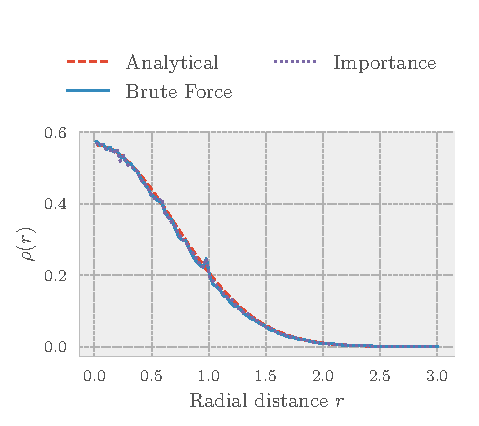
\includegraphics[width=.8\linewidth]{figures/density1.pdf}
		\subcaption{Approximation of onebody density using Metropolis brute force sampling vs analytical(kilde)}
		\label{fig:sfig1}
	\end{subfigure}%
	\begin{subfigure}{\textwidth}
		\centering
		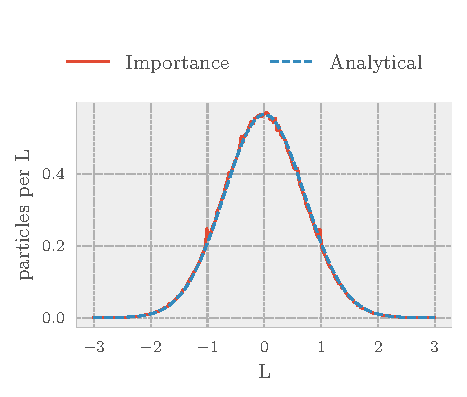
\includegraphics[width=.8\linewidth]{figures/density2.pdf}
		\subcaption{Approximation of onebody density using Metropolis importance sampling vs analytical}
		\label{fig:sfig2}
	\end{subfigure}
	\caption{One-body density of 1 boson in 1 dimmension, using $N = 1e6$ cycles, $\omega = 1$, $\alpha = 0.5$.}
	\label{fig:1 part 1 dim density}
\end{figure}

\begin{figure}
	\begin{subfigure}{\textwidth}
		\centering
		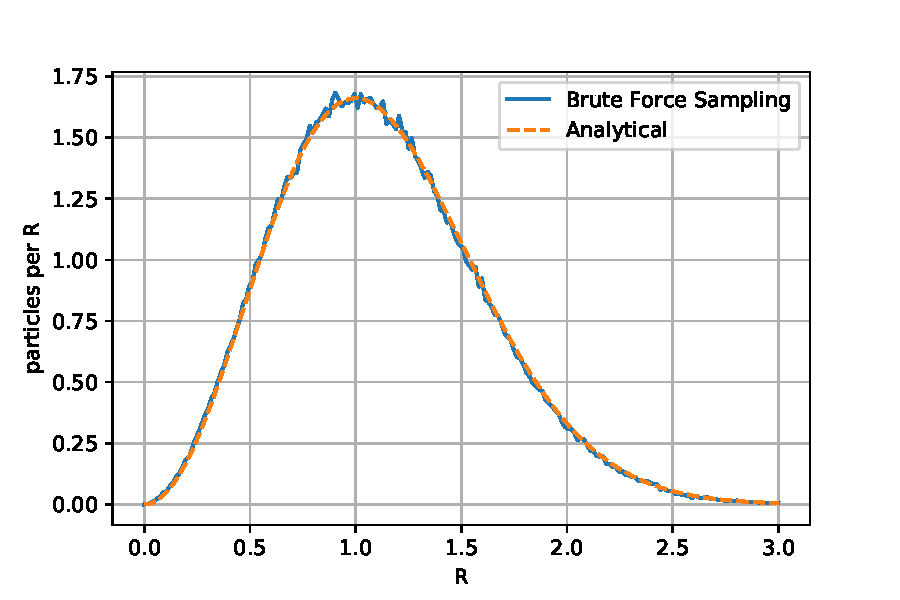
\includegraphics[width=.8\linewidth]{figures/density3.pdf}
		\subcaption{Approximation of radial onebody density using Metropolis brute force sampling vs analytical}
		\label{fig:sfig1}
	\end{subfigure}%
	\begin{subfigure}{\textwidth}
		\centering
		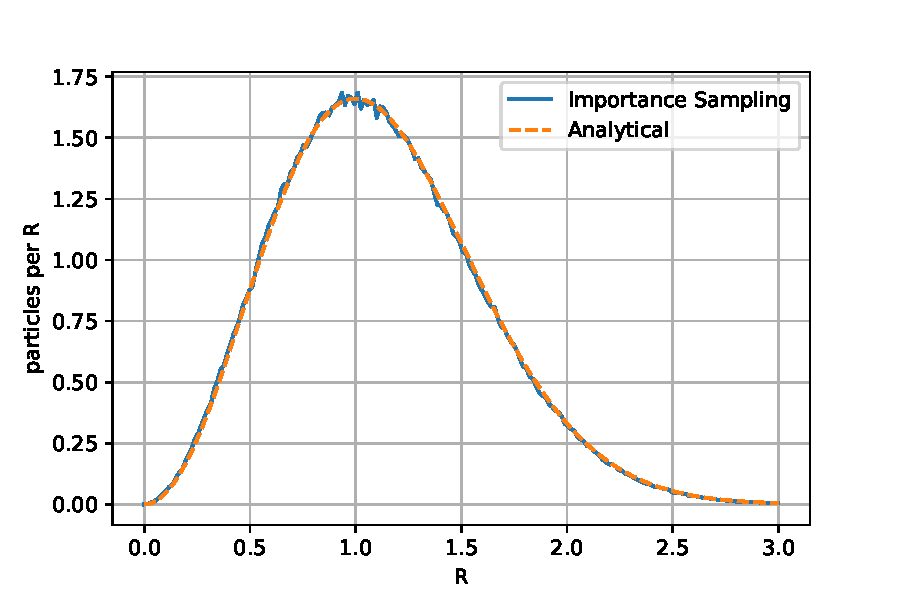
\includegraphics[width=.8\linewidth]{figures/density4.pdf}
		\subcaption{Approximation of radial onebody density using Metropolis importance sampling vs analytical}
		\label{fig:sfig2}
	\end{subfigure}
	\caption{Radial one-body density of 2 non-interacting bosons in 3 dimmensions, using $N = 1e6$ cycles, $\omega = 1$, $\alpha = 0.5$.}
	\label{fig:2 part 3 dim density}
\end{figure}

In \autoref{fig:1 part 1 dim density}  we see that both brute force sampling and importance sampling manage to approximate the onebody density derived from the non-interacting trial wave function: Aside from the statistical noise introduced by the finite number of Monte-Carlo cycles, the approximated densities follow the analytical result closely. Figure \autoref{fig:2 part 3 dim density} demonstrates that this also scales to more particles and dimensions, as seen from the radial onebody density of two particles in three dimensions. 


\subsection{Blocking of Local Energy}
\begin{figure}
	\begin{subfigure}{\textwidth}
		\centering
		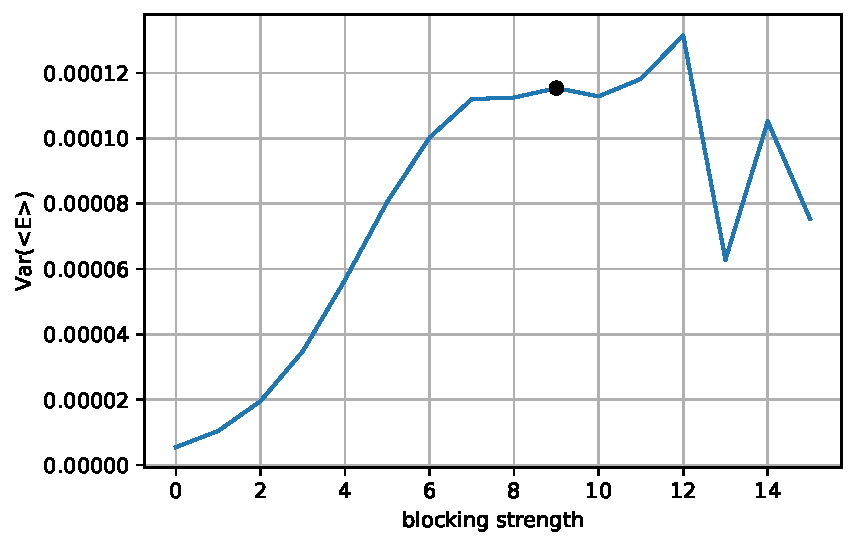
\includegraphics[width=.8\linewidth]{figures/blocking1.pdf}
		\subcaption{Brute Force Sampling}
	\end{subfigure}%
	\begin{subfigure}{\textwidth}
		\centering
		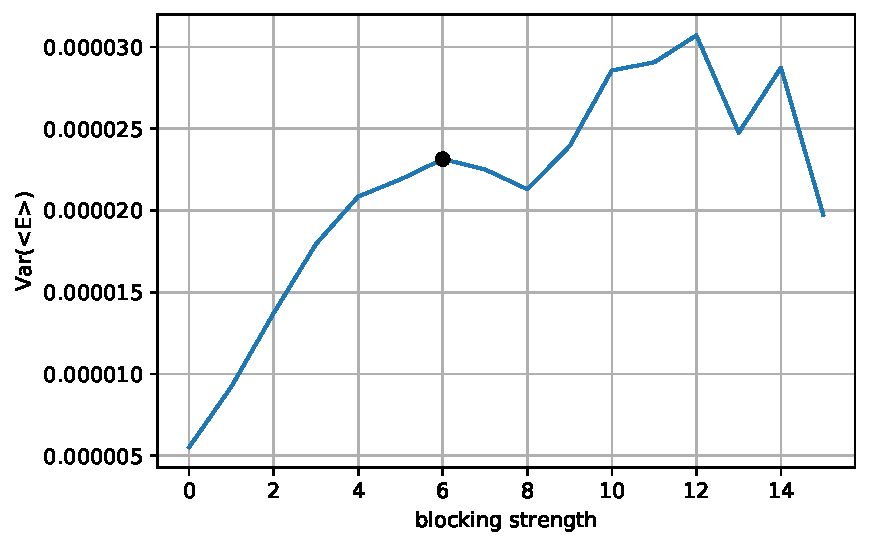
\includegraphics[width=.8\linewidth]{figures/blocking2.pdf}
		\subcaption{Importance Sampling}
	\end{subfigure}%
	\centering
	\caption{Variance of the estimate of $<E>$ using blocked values of local energy at various strengths. The data has been produced for 2 non-interacting bosons i 3 dimension, using $N = 2^{17}$ cycles, $\alpha = 0.8$, $\omega = 1$, with and without importance sampling}
	\label{fig:blocking1}
\end{figure}

In \autoref{fig:blocking1}, we see the effect of applying blocking on the local energy data before calculating the variance of the estimator (kilde). Although the local energies are sampled from an approximately correct distribution, as indicated by \autoref{fig:2 part 3 dim density}, the data is produced by moving a single electron at a time. Moreover, the move may even be rejected by the metropolis algorithm. Thus, the data is highly correlated, causing an underestimation of the variance as seen for the unblocked data(blocking strength $0$). After repeated blocking, the variance stabilizes when the data is approximately uncorrelated. Note that this happens at different strengths of blocking with brute force sampling and with importance sampling. This indicates that latter method creates data that are less correlated that when brute force is used. This makes sense, as importance sampling uses additional information from the wave function and explores the space of states more efficiently than brute force. \autoref{fig:blocking1} shows that the variance stabilizes for strength equal $6$ for importance sampling, rather than $9$ for brute force. This grants us 8 times the effective amount of data and thus a smaller variance of the estimator.

\begin{figure}
	\centering
	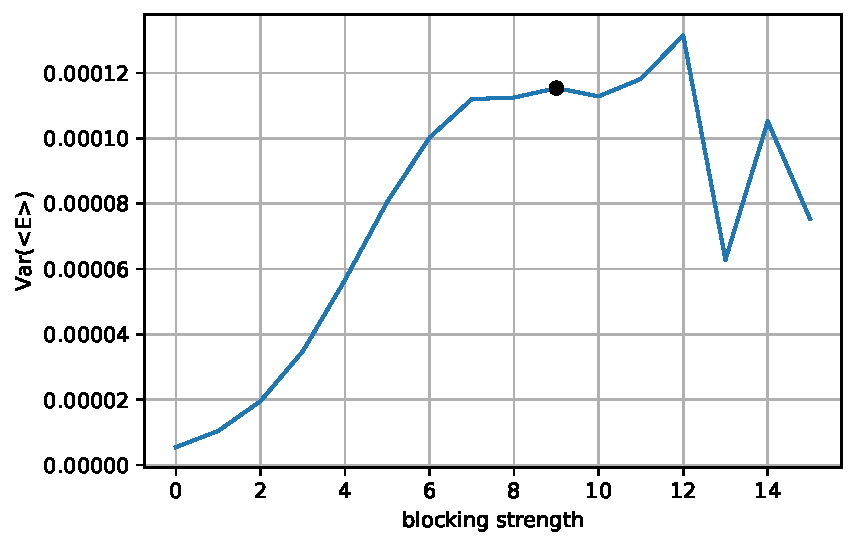
\includegraphics[width=.8\linewidth]{figures/blocking1.pdf}
	\caption{Variance of the estimate of $<E>$ using blocked values of local energy at various strengths. The data has been produced for 2 non-interacting bosons i 3 dimension, using $N = 2^{17}$ cycles, $\alpha = 0.8$, $\omega = 1$, with and without importance sampling}
	\label{fig:blocking3}
\end{figure}



\subsection{Interacting Potentials}
\subsection{Local Energy}
\subsection{Optimal Parameter \(\alpha\)}
\subsection{Onebody Density}

